\documentclass[border=6pt]{standalone}
\usepackage{fontspec}
\IfFileExists{fonts/times.ttf}{
  \setmainfont{times.ttf}[Path=fonts/,
    BoldFont=timesbd.ttf, ItalicFont=timesi.ttf, BoldItalicFont=timesbi.ttf]
}{\usepackage{mathptmx}}
\usepackage{tikz}
\usetikzlibrary{arrows.meta,positioning,fit,backgrounds,calc,shapes.geometric}
\begin{document}
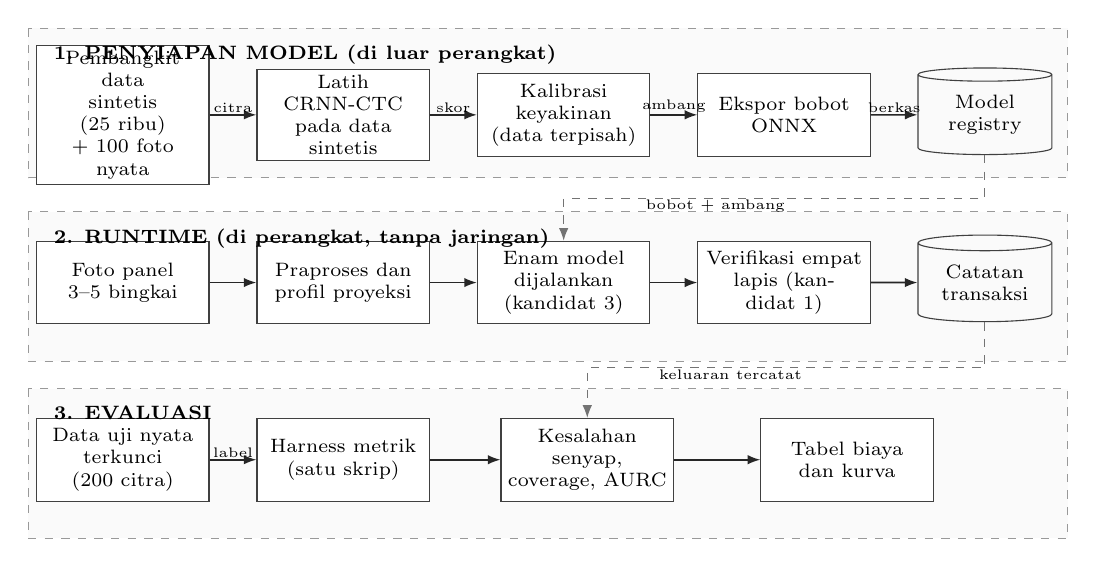
\begin{tikzpicture}[
  x=1cm, y=1cm,
  kotak/.style={rectangle, draw=black!75, fill=white, align=center,
                text width=2.05cm, minimum height=1.05cm, inner sep=2pt,
                font=\scriptsize},
  simpan/.style={cylinder, draw=black!75, shape border rotate=90,
                 aspect=0.18, minimum height=1.10cm, minimum width=1.70cm,
                 align=center, font=\scriptsize, inner sep=0pt},
  panah/.style={-{Latex[length=1.6mm]}, draw=black!85, semithick},
  panahputus/.style={-{Latex[length=1.6mm]}, draw=black!55, dashed},
  lbl/.style={font=\tiny, inner sep=0.5pt},
  judul/.style={font=\scriptsize\bfseries, anchor=north west}
]

% ---------- JALUR 1 ----------
\node[kotak] (data)  at (1.35,0.18) {Pembangkit data\\ sintetis (25 ribu)\\+ 100 foto nyata};
\node[kotak] (latih) at (4.15,0.18) {Latih CRNN-CTC\\ pada data sintetis};
\node[kotak] (kal)   at (6.95,0.18) {Kalibrasi\\ keyakinan\\ (data terpisah)};
\node[kotak] (ekspor)at (9.75,0.18) {Ekspor bobot\\ ONNX};
\node[simpan] (reg)  at (12.30,0.18) {Model\\ registry};

\draw[panah] (data)   -- node[lbl, above] {citra} (latih);
\draw[panah] (latih)  -- node[lbl, above] {skor} (kal);
\draw[panah] (kal)    -- node[lbl, above] {ambang} (ekspor);
\draw[panah] (ekspor) -- node[lbl, above] {berkas} (reg);

% ---------- JALUR 2 ----------
\node[kotak] (foto)  at (1.35,-1.95) {Foto panel\\ 3--5 bingkai};
\node[kotak] (pra)   at (4.15,-1.95) {Praproses dan\\ profil proyeksi};
\node[kotak] (model) at (6.95,-1.95) {Enam model\\ dijalankan\\ (kandidat 3)};
\node[kotak] (verif) at (9.75,-1.95) {Verifikasi empat\\ lapis (kandidat 1)};
\node[simpan] (catatan) at (12.30,-1.95) {Catatan\\ transaksi};

\draw[panah] (foto)  -- (pra);
\draw[panah] (pra)   -- (model);
\draw[panah] (model) -- (verif);
\draw[panah] (verif) -- (catatan);

% ---------- JALUR 3 ----------
\node[kotak] (gt)      at (1.35,-4.20) {Data uji nyata\\ terkunci\\ (200 citra)};
\node[kotak] (harness) at (4.15,-4.20) {Harness metrik\\ (satu skrip)};
\node[kotak] (metrik)  at (7.25,-4.20) {Kesalahan senyap,\\ coverage, AURC};
\node[kotak] (laporan) at (10.55,-4.20) {Tabel biaya\\ dan kurva};

\draw[panah] (gt)      -- node[lbl, above] {label} (harness);
\draw[panah] (harness) -- (metrik);
\draw[panah] (metrik)  -- (laporan);

% ---------- KETERGANTUNGAN ----------
\draw[panahputus] (reg.south) -- ++(0,-0.55) -| node[lbl, below, pos=0.32] {bobot + ambang} (model.north);
\draw[panahputus] (catatan.south) -- ++(0,-0.58) -| node[lbl, below, pos=0.32] {keluaran tercatat} (metrik.north);

% ---------- KOTAK JALUR ----------
\begin{scope}[on background layer]
  \draw[dashed, draw=black!40, fill=black!2] (0.15,1.28) rectangle (13.35,-0.62);
  \draw[dashed, draw=black!40, fill=black!2] (0.15,-1.05) rectangle (13.35,-2.95);
  \draw[dashed, draw=black!40, fill=black!2] (0.15,-3.30) rectangle (13.35,-5.20);
\end{scope}

\node[judul] at (0.35,1.19) {1. PENYIAPAN MODEL (di luar perangkat)};
\node[judul] at (0.35,-1.14) {2. RUNTIME (di perangkat, tanpa jaringan)};
\node[judul] at (0.35,-3.39) {3. EVALUASI};

\end{tikzpicture}
\end{document}
